
\subsection{Machine Learning Methods for Reconstruction in High Energy Physics}
\label{sec:ml_event_reconstruction_hep}


Short introductory text here stating that ML is a topic of rising interest in HEP and refer to output of ML-related papers in HEP. \cite{iml-wg-hepml-livingreview}'. \textbf{I have realized that the relevancy of this section is heavily questioned... Just cherry-pick relevant parts from here and ommit the rest I have limited space and this is not a popular science summary this background should cover necessary theory and it should cover necessary motivation for my study in my thesis, and maybe provide some context for the viewer also but nothing else. The fact that it is a rising tool of interest is still interesting to mention, but only in the contexts of why that is not simply a ''trend follower''. The rising tool of interest should be 1 or max 2 sentences.}


\textbf{text here}

\gls{ml} has become a tool of rising interest in \gls{hep}, driven by the growing complexity of detector data, the need for efficient event selection, and the search for rare signatures of physics beyond the \gls{sm}. At the same time, advances in deep-learning methods and accelerator-based computing architectures such as \glspl{gpu} have made increasingly powerful \gls{ml} and non-\gls{ml} approaches practical for scientific workflows \cite{sur2026-heterogeneous-computing}. Machine learning and deep-learning methods are not new in \gls{hep}, but the recent rapid growth of machine-learning applications in particle physics is 
\begin{wrapfigure}{r}{0.50\textwidth}
    \centering
    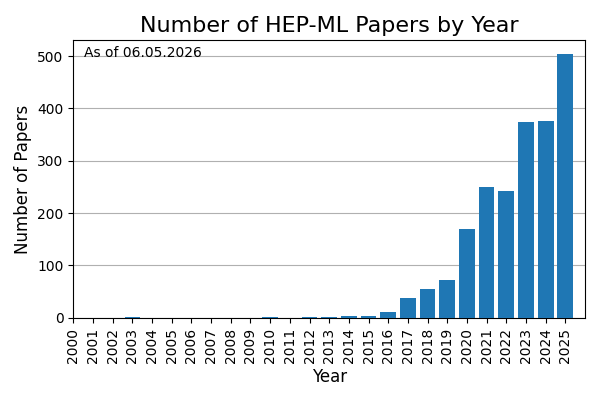
\includegraphics[width=0.48\textwidth]{config/fig/per_year.png}
    \caption{\textbf{Increase the size of labels here} Number of machine-learning-related publications on arXiv in the HEP category per year, based on the Living Review of Machine Learning for Particle Physics \cite{iml-wg-hepml-livingreview}.}
    \label{fig:ml-publications-per-year}
\end{wrapfigure}
reflected both in dedicated reviews and in the continuously updated Living Review of Machine Learning for Particle Physics  \cite{karagiorgi2021-mlnewphysics,feickert2021-livingreview,iml-wg-hepml-livingreview}. Figure \ref{fig:ml-publications-per-year} shows the trend of machine-learning-related publications within \gls{hep} significantly increasing in the last few years. 


The underlying motivation for \gls{ml} in \gls{hep} is that such tools may increase the \textit{physics reach} of experiments, meaning their ability to probe weaker signals, rarer processes, or more challenging regions of parameter space, either by improving sensitivity enabling new discoveries or by making reconstruction and selection more computationally efficient. 

\paragraph{Reconstruction} Reconstruction in \gls{hep} refers to reconstructing the physical interpretables from a measured particle event based on the detector outputs.  Modern \gls{hep} experiments produce high-dimensional and heterogeneous data, where each event may contain a variable number of detector signals distributed across several subdetectors. This makes reconstruction a quite natural application area for machine learning: the task is to transform heterogeneous low-level or intermediate detector information, such as hits, tracks, and calorimeter clusters, into physically meaningful quantities that can be used for triggering, event selection, and analysis.



A useful way to view reconstruction is as an approximate inverse problem. In simulation, a detector may be regarded as a map from an underlying particle-level event to a set of detector measurements. If the particle-level event, representing the physical ''truth'', is denoted by \(Y\), and the corresponding detector response by \(X\), the simulation can be written schematically as
\begin{equation}
    S(Y) = X ,
\end{equation}
where \(S\) represents the detector response. Reconstruction, denoted $R$,  then attempts to inverse the mapping, i.e
\begin{equation}
    R(X) \approx S^{-1}(X) = Y .
\end{equation}
In practice, this inverse is imperfect and often ambiguous, based on the fact that some information is always lost, has stochastic evolutions or only indirectly observed: detector signals have finite resolution and particles may overlap in the detector. These cases does not exclude relevance however, as it could also be useful to study these scenarios as well and infer where our tools of measurement might simply not be enough. Machine-learning-based reconstruction approaches formulate parts of this inverse problem as a learnable mapping from detector-level inputs to physics-level targets, typically using simulated events where truth information is available to us and constructing target information is completely feasible.

\subsubsection{Computational Context in Experimental High Energy Physics}

\textbf{Let Nairit read this section!}

The computational setting of \gls{hep} is also important for understanding the interest in machine-learning-based reconstruction. Large-scale \gls{hep} computing has traditionally been dominated by distributed, \gls{cpu}-based workflows. \cite{sur2026-heterogeneous-computing} This is natural because collision or fixed-target events often are, to a good approximation, independent processes, analog to the electron case of \gls{ldmx} $Z^{(k)} \perp\!\!\!\perp Z^{(\ell)}$ where $k \neq l$, following the notation introduced in Section~\ref{sec:formalism}. Simulation, reconstruction, and analysis can therefore often be parallelized over events with relatively little communication between tasks, making \gls{cpu} clusters and grid computing highly effective, somewhat bypassing an immediate need of software engineering concurrency, which explains the longevity and success of this computing paradigm within \gls{hep}.

At the same time, the wider computing landscape has shifted toward heterogeneous architectures, in particular \glspl{gpu} and other accelerator \footnote{``Accelerator'' in this context refers to specialized hardware such as \glspl{gpu} or even \gls{ml} specialized architectures such as the relatively new \gls{tpu} designed by Google that accelerate the speed of computation for applicable processes\cite{needed}}
-based systems. This development is strongly connected to modern machine learning, where many operations reduce to dense linear algebra and can be executed efficiently on massively parallel hardware, including both training and inference tasks of deep learning \gls{ml} models.

This shift creates both a challenge and an opportunity for \gls{hep}. Rule-based reconstruction algorithms have often been designed around detector-specific logic and sequential or iterative procedures. Such algorithms can be highly effective, but they may be difficult to port efficiently to accelerator hardware and may scale poorly with detector occupancy. Machine-learning models, by contrast, often express reconstruction as a fixed sequence of tensor operations, making inference naturally suited to \glspl{gpu} or other accelerator architectures. 

\subsubsection{MLPF, a Recent Example of ML-based Reconstruction in HEP}

All of the above stated reasons creates a modern context that make up the underlying motivations behind the \gls{mlpf} reconstruction method, designed for the \gls{cms} experiment and the incoming \textit{high luminosity phase} of the \gls{lhc}. The original \gls{mlpf} study published in 2021 used a graph-neural-network-based architecture for efficient particle-flow reconstruction in high-pile-up conditions \cite{pata2021-mlpf}. The latest implementation from early 2026 demonstrates a transformer-based \gls{mlpf} algorithm integrated into the \gls{cms} reconstruction software and evaluated on both simulation and collision data \cite{pata2026-mlpf}. In the latter study, modern hardware, transformer-based computational architectures and recent progress of  the transformer architecture are explicitly part of the motivation for scalable reconstruction in high-dimensional, variable-size event data.

The \gls{mlpf} showcases the motivation for \gls{ml} based reconstruction quite perfectly combining all of the above stated reasons for why \gls{ml} methods have sparked an interest. The \gls{mlpf} uses the modern model architecture, compute is accelerated with modern hardware, the method shows promise of improved speed of compute, resolution of reconstruction and it is motivated by the context of \gls{lhc} high luminosity phase, which will increase complexity with a much higher rate of pile-up.

For the purpose of this thesis, the most relevant role of machine learning is therefore not only as a final classifier that separates signal-like and background-like events, but as a possible reconstruction method. Traditional reconstruction algorithms are often built from physics-motivated rules and detector-specific heuristics. Such methods remain essential, but they may become difficult to optimize in environments with high occupancy, irregular detector geometry, or overlapping detector signatures. Machine-learning-based reconstruction instead attempts to learn parts of the reconstruction mapping $R(X) \approx S^{-1}(X) = Y$ directly from simulated or measured data. It is also important to understand that rule-based and \gls{ml} reconstruction is not either/or, they are the most effective when they work in junction and complement each other. The \gls{mlpf} model takes some object-level inputs that are the results of rule-based reconstruction intermediate outputs such as clusters and particle candidates, in which the \gls{ml}-based \gls{mlpf} can utilize for stronger inference results \cite{pata2021-mlpf}. 

\subsubsection{The GNN and the Transformer under Pile-Up Conditions}

\gls{ml}-based methods are perhaps the most relevant under pile-up conditions, where detector hits from several particles or interactions may overlap and where the association between detector activity and the underlying particle origin becomes ambiguous. In this setting, a model that operates directly on hit-level or object-level detector information may provide additional information beyond a purely rule-based reconstruction, for example by assigning hit-level probabilities or by learning correlations that may be difficult to capture manually with code. One must still remember however that \gls{ml}-methods are certainly also based on ''rules'' in the end, the strength of these methods in this context lie in that their discovery of efficient, or even \textit{optimal} ''rules'', are somewhat automatic and a researcher can explore the space of solutions efficiently.

Architectures such as \glspl{gnn} and \textit{transformer} are particularly well suited to this type of problem because they can operate on variable-size collections of detector objects and learn correlations between them without requiring the data to be arranged on a regular grid. This is important for particle detectors, where the relevant information is often distributed over irregular detector geometries and across multiple subdetectors. By contrast, architectures such as \glspl{cnn} are naturally adapted to regularly spaced image-like data and therefore impose an inductive bias that is not always well matched to detector readout. Graph-based models instead allow calorimeter hits, clusters, tracks, or other detector objects to be represented as nodes, with edges describing geometrical proximity or learned relationships. Transformers provide a related approach but it uses different analogies than nodes and edges. 

In this thesis, the same general motivation is applied to the \gls{ldmx} setting. The aim is not to perform full general-purpose particle-flow reconstruction, as in \gls{cms}, but to build and study a reconstruction platform for identifying electron-induced activity in the electromagnetic calorimeter down to hit-level statistics, especially under pile-up conditions. This is the regime where reconstruction ambiguities are expected to be most relevant, and where machine-learning methods may offer the largest benefit over rule-based approaches.

\textbf{This is kind of outdated, should I include all of this or not?} The rest of this subsection introduces the machine-learning context needed for the reconstruction study in this thesis. First, the existing rule-based reconstruction chain in \gls{ldmx} is reviewed, with emphasis on clustering, particle-flow-inspired reconstruction, and the distinction between online and offline reconstruction. The existing machine-learning-based veto strategy in \gls{ldmx} is then briefly discussed, since it represents an already planned use of machine learning in the experiment \textbf{not relevant for my study?}. The subsection then turns to machine-learning-based reconstruction in \gls{cms}, in particular the development of \gls{mlpf}, which provides a useful point of comparison for the approach studied here. Finally, the basic ideas behind \glspl{gnn} and transformers are introduced and compared. These architectures form the methodological basis for representing calorimeter hits and other detector objects as unordered sets of nodes or tokens, allowing event reconstruction to be formulated as a learnable mapping from detector-level inputs to physics-level targets.

\textbf{Further motivation of why not to use CNN to use somewhere maybe:}

This representation preserves individual detector objects rather than
projecting the event to an image. The number of hits is event dependent, the
\gls{ecal} is 3D, and overlapping showers need not be aligned
with a fixed rasterization. Moreover, trigger-pad-track information is not an
\gls{ecal} pixel quantity. Sets, learned graphs and attention-based token
sequences provide natural ways of relating these heterogeneous objects while
remaining insensitive to an arbitrary ordering of the input rows.















\subsection{things that I want to include but have maybe not found a suitable place for yet}

* \gls{gnn}, Transformer work with unordered sets of input compared to CNN that is on a regular grid. We are using different detectors and different objects and the ECal has a hexagonal grid and all of this adds to difficulty of using CNNs. 

Briefly mention clustering and reconstruction methods that LDMX has already implemented and plans to potentially use. Describe these existing LDMX reconstruction approaches very shortly, and these are based on other methods developed at \gls{cms} CERN already (clustering CLUE, particle flow PF), where the the detector design such as the ECal is the inspiration and what LDMX is based at giving that the LDMX detector is a so-called "sibling detector".

Briefly mention that machine learning approaches have been explored by previous thesis students testing CNN, \gls{gnn} and even RNN, and reference these.

Briefly mention and explain and a particle-net (\gls{gnn}) implementation that was made for ML-based Veto in LDMX (explain what a veto is).


\subsubsection{ML-based Reconstruction in CMS}

\textbf{comment: This is a title that I think was interesting when I thought to explain particlenet, though I have come to the conclusion with my supervisor that explaining and detailing other reconstruction methods is not directly relevant to my work and there is not enough time to expand my analysis or to explain all of this in detail I can only briefly mention it for useful context for the reader and to motivate my study compared to previous students.}
